\maketitle

\begin{abstract}
\noindent This experiment is concerned with the heterogeneous equilibrium between two phases in a system of two components, 
The particular system to be studied is acetone--chloroform at \qty{1}{\atm} pressure. 
This system exhibits a strong negative deviation from Raoult's law, resulting in the existence of a maximum boiling point.\thanks{Transcribed from \textcite{nibler14}.}
\end{abstract}

\section{Theory}
\label{sec:theory}

For a system of two components (\(A\) and \(B\)), we have from the phase rule,\cite{atkins94}
\begin{equation}
	F = C - P + 2 = 4 - P
	\label{eq:phase_components}
\end{equation}
where \(C\) is the number of \emph{components},\sidenote{The minimum number of chemical constituents necessary to define the composition of every phase in the system at equilibrium.} \(P\) is the number of \emph{phases},\sidenote{The number of physically differentiable parts of the system at equilibrium.} and \(F\) is the \emph{variance} or number of \emph{degrees of freedom}.\sidenote{The number of intensive variables pertaining to the system that can be independently varied at equilibrium without altering the number or kinds of phases present.}

When a single phase is present, the pressure \(p\), the temperature \(T\), and the composition \(X_B\)\sidenote{The mole fraction of component \(B\).} of that phase can be varied independently; thus, a single-phase two-component system at equilibrium is defined, except for its size,\sidenote{The complete definition of the system would of course also include its shape, description of surfaces, specification of fields, etc.; ordinarily these have negligible effects as far as our present discussion is concerned.} by a point in a three-dimensional plot in which the coordinates are the intensive variables \(p\), \(T\), and \(X_B\) (see \cref{fig:phase_diagram}).
When two phases, \eg, liquid \(L\) and vapor \(V\), are present at equilibrium, there are four variables, but only two of them can be independently varied. 
Thus, if \(p\) and \(T\) are specified, \(X_{B,L}\) and \(X_{B,V}\)\sidenote{The mole fractions of \(B\) in \(L\) and \(V\).} are fixed at their \emph{limiting} values (\(X_{B,L}^0\) and \(X_{B,V}^0\)) for the respective phases at this \(p\) and \(T\). 
The loci of points \(X_{B,L}^0(p, T)\) and \(X_{B,V}^0(p, T)\) constitute two surfaces, shown in \cref{fig:vl_diagram}. 
The shaded region between them may be interpreted as representing the coexistence of two phases \(L\) and \(V\) \emph{if}, in this region, \(X_B\) is interpreted as a mole fraction of \(B\) \emph{for the system as a whole}. 
Within the two-phase region, \(X_B\) is \emph{not} to be regarded as one of the intensive variables constituting the variance.\sidenote{Although, in a single-phase region, it is indeed one of these variables.}
In a two-phase region, the value of \(X_B\) determines the relative proportions of the two phases in the system; as \(X_B\) varies from \(X_{B,L}^0\) to \(X_{B,V}^0\), the molar proportion \(x_V\) of the vapor phase varies from zero to unity:
\begin{equation}
	x_V = 1 - x_L = \frac{X_B - X_{B,L}^0}{X_{B,V}^0 - X_{B,L}^0}
	\label{eq:vapor_proportion}
\end{equation}

\begin{figure}[htb]
	\documentclass{standalone}
\usepackage{pgfplots,amsmath}
\pgfplotsset{compat=1.18}
\usetikzlibrary{math,arrows.meta}

\begin{document}


\pgfplotsset{
  % height = 0.7\textwidth,
  width = 0.9\textwidth,
  scale only axis,
}

\newcommand{\vertLineFromPoint}[1]{
  \draw[dashed] 
	(#1) -- (#1|-{0,\pgfkeysvalueof{/pgfplots/ymin}})
}

\begin{tikzpicture}
	\begin{axis}[
	clip=true,
	xtick={1},
	xticklabels={$T_c$},
	xmin=-0.1, xmax=1.1, 
	ymin=-1.1, ymax=1.1,
	]
	
	\addplot [mark=none,smooth,thick] coordinates {
				(0.0, 	-1.0)
				(0.19, 	-0.9)
				(0.36, 	-0.8)
				(0.4375, -0.75)
				(0.51, 	-0.7)
				(0.64,	-0.6)
				(0.75,	-0.5)
				(0.84, 	-0.4)
				(0.91, 	-0.3)
				(0.9375, -0.25)
				(0.96, 	-0.2)
				(.99,	-0.1)
				(1.0, 	0.0) 
				(.99,	0.1)
				(0.96, 	0.2)
				(0.9375, 0.25)
				(0.91, 	0.3)
				(0.84, 	0.4)
				(0.75,	0.5)
				(0.64,	0.6)
				(0.51, 	0.7)
				(0.4375, 0.75)
				(0.36, 	0.8)
				(0.19, 	0.9)
				(0, 	1)};	
	
	\draw [dashed] (1.0, 0.0) -- (1.0, -1.1);		
	
	\end{axis}
\end{tikzpicture}

\end{document}

	\caption{Schematic three-dimensional vapor--liquid equilibrium diagram for a two-component system obeying Raoult's law.}
	\label{fig:phase_diagram}
\end{figure}


\Cref{fig:vl_diagram} is drawn for the special case of two components that form a complete range of \emph{ideal solutions}, \ie, solutions that obey Raoult's law with respect to both components at all compositions. 
According to this law, the vapor pressure\sidenote{Or the partial pressure in the vapor.} of a component at a given temperature \(T_1\) is proportional to its mole fraction in the liquid. 
Thus in \cref{fig:vl_diagram}, the light  dashed lines representing the partial pressures \(p_A\) and \(p_B\) and the total vapor-pressure line \sidenote{\(L\), joining \(p_A\) and \(p_B\)} are straight lines when plotted against the liquid composition. 
However, the total vapor pressure as plotted agains the \emph{vapor} composition is not linear. 
The curved line \(V\), joining \(p_A\) and \(p_B\), is convex downward, lying \emph{below} the straight line on the constant-temperature section; its slope has everywhere the same sign as the slope of \(L\). 

The vapor pressures \(p_A^0\) and \(p_B^0\) of the pure liquids increase with temperature\sidenote{In accordance with the Clapeyron equation.} as indicated by the curses joining \(p_A^0\) with \(p_A^0\prime\) and \(p_B^0\) with \(p)_B^0\prime\).
At a constant pressure, say \qty{1}{\atm}, the boiling points of the pure liquids are indicated as \(T_A^0\) and \(T_B^0\). The boiling point of the solution, as a function of \(X_{B,L}\) or \(X_{B,V}\), is represented by the curve \(L^*\) or \(V^*\) joining these two points. 
Neither curve is in general a straight line. 
If Raoult's law is obeyed, both are convex upward in temperature, the vapor curve lying above the liquid curve in temperature and being the more convex. 

In most binary liquid--vapor systems, Raoult's law is a good approximation for a component only when its mole fraction is close to unity. 
Large deviations from this law are commonplace for the dilute component or for both components when the mole fraction of neither is close to unity. 
If, at a given temperature, the vapor pressure of a solution is higher than that predicted by Raoult's law, the system is said to show a \emph{positive deviation} from that law. 
For such a system, the boiling-point curve \(L^*\) at constant pressure is usually convex downward in temperature. 
If, at a given temperature, the vapor pressure of the solution is lower than that predicted by Raoult's law, the system is said to show a \emph{negative deviation}; in this case, the curve \(L^*\) is more convex upward. 
These deviations from Raoult's law are often ascribed to differences between the ``heterogeneous'' molecular attractions\sidenote{\ch{A-B}} and ``homogeneous'' attractions. \sidenote{\ch{A-A} and \ch{B-B}}
Thus, the existence of a positive deviation implies that homogeneous attractions are stronger than heterogeneous attractions, and a negative deviation implies the reverse. 
This interpretation is consistent with the fact that positive deviations are usually associated with positive heats of mixing and volume expansions on mixing, while negative deviations are usually associated with negative heats and volume contractions. 

\begin{figure}[htb]
	\centering
	\subfloat[\label{fig:raoult_dev_pos}Chloroform--acetone mixture]{
		\documentclass{standalone}
\usepackage{pgfplots,pgfplotstable,amsmath}
\pgfplotsset{compat=1.18}
\usetikzlibrary{math,arrows.meta}

\begin{document}
\newcommand{\vertLineFromPoint}[1]{
  \draw[dashed] 
	(#1) -- (#1|-{0,\pgfkeysvalueof{/pgfplots/ymin}})
}
% \tikzset{
%   every pin edge/.style={thick,<-,>=Stealth},
% }
\pgfplotsset{
  % height = 0.4\textwidth,
  width = 0.4\textwidth,
  scale only axis,
}
\pgfplotstableset{col sep=comma}

\pgfplotstableread{figures/raoult_dev_pos_p.csv}\posPtable
\pgfplotstableread{figures/raoult_dev_pos_t.csv}\posTtable
% \pgfplotstabletypeset{\posPtable}

\begin{tikzpicture}
	  \begin{axis}[
	  ylabel={$p$},
	  xlabel={$X_B \rightarrow$},
	  ytick=\empty,
	  xtick={0,1},
	  xticklabels={$A$,$B$},
	  xmin=0, xmax=1]
	  \addplot [smooth,blue,thick] 
		  table [x=x1, y=Pressure] {\posPtable} 
		  node [above,yshift=6,pos=0.20] {$V$};  
	  \addplot+ [mark=none,smooth,thick] 
		  table [x=y1, y=Pressure] {\posPtable} 
		  node [below,yshift=-6,pos=0.28] {$L$};  
	  \end{axis}
\end{tikzpicture}

\begin{tikzpicture}
	  \begin{axis}[
	  ylabel={$T$},
	  xlabel={$X_B \rightarrow$},
	  ytick=\empty,
	  xtick={0,1},
	  xticklabels={$A$,$B$},
	  xmin=0, xmax=1]
	  \addplot [smooth,blue,thick] 
		  table [x=x1, y=Temperature] {\posTtable} 
		  node [below,yshift=-8,pos=0.28] {$L^*$};  
	  \addplot+ [mark=none,smooth,thick] 
		  table [x=y1, y=Temperature] {\posTtable} 
		  node [above,yshift=8,pos=0.25] {$V^*$};  
	  \end{axis}
\end{tikzpicture}

\end{document}
	}\\
	\subfloat[\label{fig:raoult_dev_neg}Chloroform--methanol mixture]{
		\documentclass{standalone}
\usepackage{pgfplots,pgfplotstable,amsmath}
\pgfplotsset{compat=1.18}
\usetikzlibrary{math,arrows.meta}

\begin{document}
\newcommand{\vertLineFromPoint}[1]{
  \draw[dashed] 
	(#1) -- (#1|-{0,\pgfkeysvalueof{/pgfplots/ymin}})
}
% \tikzset{
%   every pin edge/.style={thick,<-,>=Stealth},
% }
\pgfplotsset{
  % height = 0.4\textwidth,
  width = 0.4\textwidth,
  scale only axis,
}
\pgfplotstableset{col sep=comma}

\pgfplotstableread{figures/raoult_dev_neg_p.csv}\negPtable
\pgfplotstableread{figures/raoult_dev_neg_t.csv}\negTtable

\begin{tikzpicture}
	  \begin{axis}[
	  ylabel={$p$},
	  xlabel={$X_B \rightarrow$},
	  ytick=\empty,
	  xtick={0,1},
	  xticklabels={$A$,$B$},
	  xmin=0, xmax=1]
	  \addplot [smooth,blue,thick] 
		  table [x=x1, y=Pressure] {\negPtable} 
		  node [above,yshift=6,pos=0.28] {$V$};  
	  \addplot+ [mark=none,smooth,thick] 
		  table [x=y1, y=Pressure] {\negPtable} 
		  node [below,yshift=-6,pos=0.20] {$L$};  
	  \end{axis}
\end{tikzpicture}

\begin{tikzpicture}
	  \begin{axis}[
	  ylabel={$T$},
	  xlabel={$X_B \rightarrow$},
	  ytick=\empty,
	  xtick={0,1},
	  xticklabels={$A$,$B$},
	  xmin=0, xmax=1]
	  \addplot [smooth,blue,thick] 
		  table [x=x1, y=Temperature] {\negTtable} 
		  node [below,yshift=-8,pos=0.32] {$L^*$};  
	  \addplot+ [mark=none,smooth,thick] 
		  table [x=y1, y=Temperature] {\negTtable} 
		  node [above,yshift=8,pos=0.30] {$V^*$};  
	  \end{axis}
\end{tikzpicture}

\end{document}
	}
	\caption{Schematic vapor-pressure and boiling-point diagrams for systems showing \protect\subref{fig:raoult_dev_pos} a strong positive deviation and \protect\subref{fig:raoult_dev_neg} a strong negative deviation from Raoult's law.}
	\label{fig:raoult_deviations}
\end{figure}

In many cases, the deviations are large enough to result in maxima or minima in the vapor-pressure and boiling-point curves, as shown in \cref{fig:raoult_deviations}. 
Systems for which the boiling-point curves have a minimum (\cref{fig:raoult_dev_pos}) include methanol--chloroform, water--ethanol, and benzene--ethanol; systems with a maximum (\cref{fig:raoult_dev_neg}) include acetone--chloroform and hydrogen-chloride--water. 
At a maximum or a minimum, the compositions of the liquid and the vapor are the same; accordingly, there is a \emph{point of tangency} of the curves \(L\) and \(V\) and of the curves \(L^*\) and \(V^*\) at the maximum or minimum. 
At every value of \(X_B\), the slope of \(V\) (or \(V^*\)) has the same sign as the slope of \(L\) (or \(L^*\)); one is zero where, and only where, the other is zero, at the point of tangency.\sidenote{A common error in curves of this kind, found even in some textbooks, is to draw a kink or cusp---a point of discontinuity of slope---in one or both curves at the point of tangency; both curves are, in fact, smooth and have continuous derivatives.}

\begin{marginfigure}
	\documentclass{standalone}
\usepackage{pgfplots,pgfplotstable,amsmath}
\pgfplotsset{compat=1.18}
\usetikzlibrary{math,arrows.meta}

\begin{document}
\newcommand{\vertLineFromPoint}[1]{
  \draw[dashed] 
	(#1) -- (#1|-{0,\pgfkeysvalueof{/pgfplots/ymin}})
}
% \tikzset{
%   every pin edge/.style={thick,<-,>=Stealth},
% }
\pgfplotsset{
  % height = 0.4\textwidth,
  width = 0.95\textwidth,
  scale only axis,
}
\pgfplotstableset{col sep=comma}

\pgfplotstableread{figures/vl_diagram.csv}\vltable

\begin{tikzpicture}
	  \begin{axis}[
	  clip=false,
	  legend entries={Vapor, Liquid},
	  legend pos=north west,
	  ylabel={$T$},
	  ytick=\empty,
	  xtick={0,1},
	  xticklabels={$A$,$B$},
	  xmin=0, xmax=1]
	  \addplot+ [mark=none,smooth] 
		  table [x=x1, y=Temperature] {\vltable};
	  \addplot+ [mark=none,smooth] table [x=y1, y=Temperature] {\vltable};
	  \addplot+ [mark=none,smooth,very thick,red,-Stealth,
				  y filter/.expression={y<95 || y>100 ? nan : y},
				] 
				table [x=y1, y=Temperature, skip coords between index={0}{22}] {\vltable};
	  \addplot+ [mark=none,smooth,very thick,blue,-Stealth,
				y filter/.expression={y<95 || y>100 ? nan : y},
					] 
				  table [x=x1, y=Temperature, skip coords between index={0}{22}] {\vltable};
	  \addlegendentry{Vapor}
	  \addlegendentry{Liquid}
	  
	  \coordinate (Xl1) at (axis cs:0.65, 95.6218);
	  \coordinate (Xg1) at (axis cs:0.412386, 95.6218);
	  \coordinate (Xl2) at (axis cs:0.75, 98.5294);
	  \coordinate (Xg2) at (axis cs:0.533324, 98.5294);
	  
	  \vertLineFromPoint{Xl1};
	  \vertLineFromPoint{Xg1};
	  \vertLineFromPoint{Xl2};
	  \vertLineFromPoint{Xg2};
	  
	  \draw (Xl1) -- (Xg1);
	  \draw (Xl2) -- (Xg2);
	  
	  \node [coordinate, pin=274:{$X_{B,L1}$}] at (axis cs:0.65,\pgfkeysvalueof{/pgfplots/ymin}) {};
	  \node [coordinate,pin=below left:{$X_{B,V1}$}] at (axis cs:0.412386,\pgfkeysvalueof{/pgfplots/ymin}) {};
	  \node [coordinate,pin=below right:{$X_{B,L2}$}] at (axis cs:0.75,\pgfkeysvalueof{/pgfplots/ymin}) {};
	  \node [coordinate,pin=266:{$X_{B,V2}$}] at (axis cs:0.533324,\pgfkeysvalueof{/pgfplots/ymin}) {};
	  
	  \end{axis}
\end{tikzpicture}

\end{document}
	\caption{Variation of liquid and vapor compositions during distillation of a system with small positive deviations from Raoult's law.}
	\label{fig:vl_diagram}
\end{marginfigure}
Liquid--vapor phase diagrams, and boiling-point diagrams in particular, are of importance in connection with \emph{distillation}, which usually has as its objective the partial or complete separation of a liquid solution into its components. 
Distillation essentially consists of boiling the solution and condensing the vapor into a separate receiver. 
A simple ``one-plate'' distillation of a binary system having no maximum or minimum in its boiling-point curve can be understood by reference to \cref{fig:vl_diagram}. 
Let the mole fraction of \(B\) in the initial solution be represented by \(X_{B, L1}\). 
When this is boiled and a small portion of vapor is condensed, a drop of distillate is obtained, with mole fraction \(X_{B,V1}\). 
Since this is richer in \(A\) than is the residue in the flask, the residue becomes slightly richer in \(B\), as represented by \(X_{B,L2}\). 
The next drop of distillate, \(X_{B,L2}\), is richer in \(B\) than was the first drop. 
If the distillation is continued until all the residue has boiled away, the last drop to condense will be virtually pure \(B\). 
To obtain a substantially complete separation of the solution into pure \(A\) and \(B\) by distillations of this kind, it is necessary to separate the distillate into portions by changing the receiver during the distillation, then subsequently to distill the separate proportions in the same way, and so on, a very large number of successive distillations being required. 
The same result can be achieved in a single distillation by use of a fractionating column containing a large number of ``plates''; discussion of the operation of such a column is beyond the scope of this book. 
If there is a maximum in the boiling-point curve (\cref{fig:raoult_dev_neg}), the composition of vapor and residue do not approach pure \(A\) or pure \(B\), but rather the composition corresponding to the maximum. 
A mixture of this composition will distill without change in composition and is known as a \emph{constant-boiling mixture} or \emph{azeotrope}. 
These terms are also applied to a mixture with a minimum boiling point. 
Azeotropes are important in chemical technology. 
Occasionally they are useful;\sidenote{As in constant-boiling aqueous hydrochloric acid, used as an analytical standard.} often they are nuisances.\sidenote{As in the case of the azeotrope of \qty{95}{\percent} ethanol with \qty{5}{\percent} water, the existence of which prevents preparation of absolute ethanol by direct distillation of dilute solutions of ethanol in water}
Extensive lists of azeotropes have been compiled.\cite{horsley1973azeotropic}

\subsection{Method}
\label{subs:method}

A boiling-point curve can be constructed from data obtained in actual distillations in an ordinary ``one-plate'' distilling apparatus. 
Small samples of the distillate are taken directly from the condenser, after which small samples of the residue are withdrawn with a pipette. 
The samples of distillate and residue are analyzed, and their compositions are plotted on a boiling-point diagram against the temperatures at which they were taken. 
In the case of the distillate, the temperature to be plotted should be recorded at the point where the distillation is stopped to take the sample of residue. 

For analysis of the samples, a physical method is often preferable to chemical methods. 
Chemical analysis is usually appropriate only when a sample titration of each sample is involved, as in the case of the system \ch{HCl-H2O}. 
If a physical property is chosen as the basis for an analytical method, it should be one which changes significantly and sensitively over the entire composition range to be studied. 
For the system acetone--chloroform, the use of a refractometer is recommended for analyzing the specimens.
In \cref{tab:ri_table}, the refractive index is given at various compositions for this system. 

\begin{table*}[t]
	\centering
	\begin{tabular}{@{}SS|SS|SS|SS}
	\toprule
		{\(n_D^{25}\)} & \%\ch{CHCl3} & {\(n_D^{25}\)} & \%\ch{CHCl3} & {\(n_D^{25}\)} & \%\ch{CHCl3} & {\(n_D^{25}\)} & \%\ch{CHCl3} \\ \midrule
		1.3562 &  0.00 & 1.3780 & 23.50 & 1.4000 & 47.55 & 1.4220 &  72.85 \\ 
		1.3570 &  0.75 & 1.3790 & 24.60 & 1.4010 & 48.70 & 1.4230 &  74.10 \\ 
		1.3580 &  1.75 & 1.3800 & 25.65 & 1.4020 & 49.80 & 1.4240 &  75.30 \\ 
		1.3590 &  2.75 & 1.3810 & 26.70 & 1.4030 & 50.90 & 1.4250 &  76.50 \\ 
		1.3600 &  3.80 & 1.3820 & 27.80 & 1.4040 & 52.00 & 1.4260 &  77.70 \\ 
		1.3610 &  4.85 & 1.3830 & 28.85 & 1.4050 & 53.10 & 1.4270 &  78.95 \\ 
		1.3620 &  5.90 & 1.3840 & 29.95 & 1.4060 & 54.20 & 1.4280 &  80.20 \\ 
		1.3630 &  7.00 & 1.3850 & 31.00 & 1.4070 & 55.30 & 1.4290 &  81.40 \\ 
		1.3640 &  8.10 & 1.3860 & 32.05 & 1.4080 & 56.45 & 1.4300 &  82.65 \\ 
		1.3650 &  9.20 & 1.3870 & 33.15 & 1.4090 & 57.60 & 1.4310 &  83.90 \\ 
		1.3660 & 10.30 & 1.3880 & 34.25 & 1.4100 & 58.75 & 1.4320 &  85.15 \\
		1.3670 & 11.40 & 1.3890 & 35.30 & 1.4110 & 59.90 & 1.4330 &  86.40 \\
		1.3680 & 12.50 & 1.3900 & 36.40 & 1.4120 & 61.05 & 1.4340 &  87.70 \\
		1.3690 & 13.60 & 1.3910 & 37.50 & 1.4130 & 62.25 & 1.4350 &  89.00 \\
		1.3700 & 14.70 & 1.3920 & 38.60 & 1.4140 & 63.40 & 1.4360 &  90.35 \\
		1.3710 & 15.80 & 1.3930 & 39.75 & 1.4150 & 64.55 & 1.4370 &  91.65 \\
		1.3720 & 16.90 & 1.3940 & 40.85 & 1.4160 & 65.75 & 1.4380 &  93.00 \\
		1.3730 & 18.00 & 1.3950 & 42.00 & 1.4170 & 66.90 & 1.4390 &  94.35 \\
		1.3740 & 19.10 & 1.3960 & 43.10 & 1.4180 & 68.10 & 1.4400 &  95.75 \\
		1.3750 & 20.20 & 1.3970 & 44.25 & 1.4190 & 69.30 & 1.4410 &  97.20 \\
		1.3760 & 21.30 & 1.3980 & 45.35 & 1.4200 & 70.50 & 1.4420 &  98.55 \\
		1.3770 & 22.40 & 1.3990 & 46.45 & 1.4210 & 71.70 & 1.4431 & 100.00 \\ \bottomrule
	\end{tabular}
	\caption{Refractive index versus composition for acetone--chloroform mixtures.}
	\label{tab:ri_table}
\end{table*}

\section{Safety Precautions}
\label{sec:safety}

\begin{itemize}
	\item Acetone is a skin and eye irritant Repeated exposure can cause liver, kidney, skin, and reproductive system damage. Care should be taken while handling, and appropriate PPE should always be used. 
	\item Chloroform causes eye, skin, and respiratory tract irritation. It is harmful if swallowed or inhaled and is a possible carcinogen. Take care while handling all chloroform solutions, and keep any solutions inside of a fume hood. Wear appropriate PPE at all times. 
	\item Both compounds have ``pleasant'' odors. This is not an invitation to smell the compounds, but rather a warning that a pleasant scent is not an indicator of safety. Rather, it should be taken as a warning that atmospheric concentrations are too high and your compounds are not being exhausted appropriately. If you smell either compound, check your fume hood for proper flow and sash height. 
\end{itemize}

\section{Procedure}
\label{sec:procedure}

\subsection{Required Equipment}
\label{subs:required_equipment}

\begin{itemize}
	\item (2) \qty{250}{\mL} two-neck round-bottom flask
	\item (1) \qtyrange{0}{100}{\celsius} thermometer
	\item (1) distilling head with thermometer adapter
	\item (7) condenser and rubber hose
	\item (1) vacuum adapter
	\item (2) \qty{500}{\mL} receiving flask
	\item (2) ring stands and clamps
	\item (1) heating mantle and power supply
	\item (2) Pasteur pipets
	\item (20) test tubes with stoppers
	\item (1) \qty{100}{\mL} graduated cylinder
	\item (1) refractometer
	\item clean cotton swabs
	\item acetone wash bottles
	\item \qty{300}{\mL} reagent-grade acetone
	\item \qty{200}{\mL} reagent-grade chloroform
\end{itemize}

\begin{figure}
	\centering
	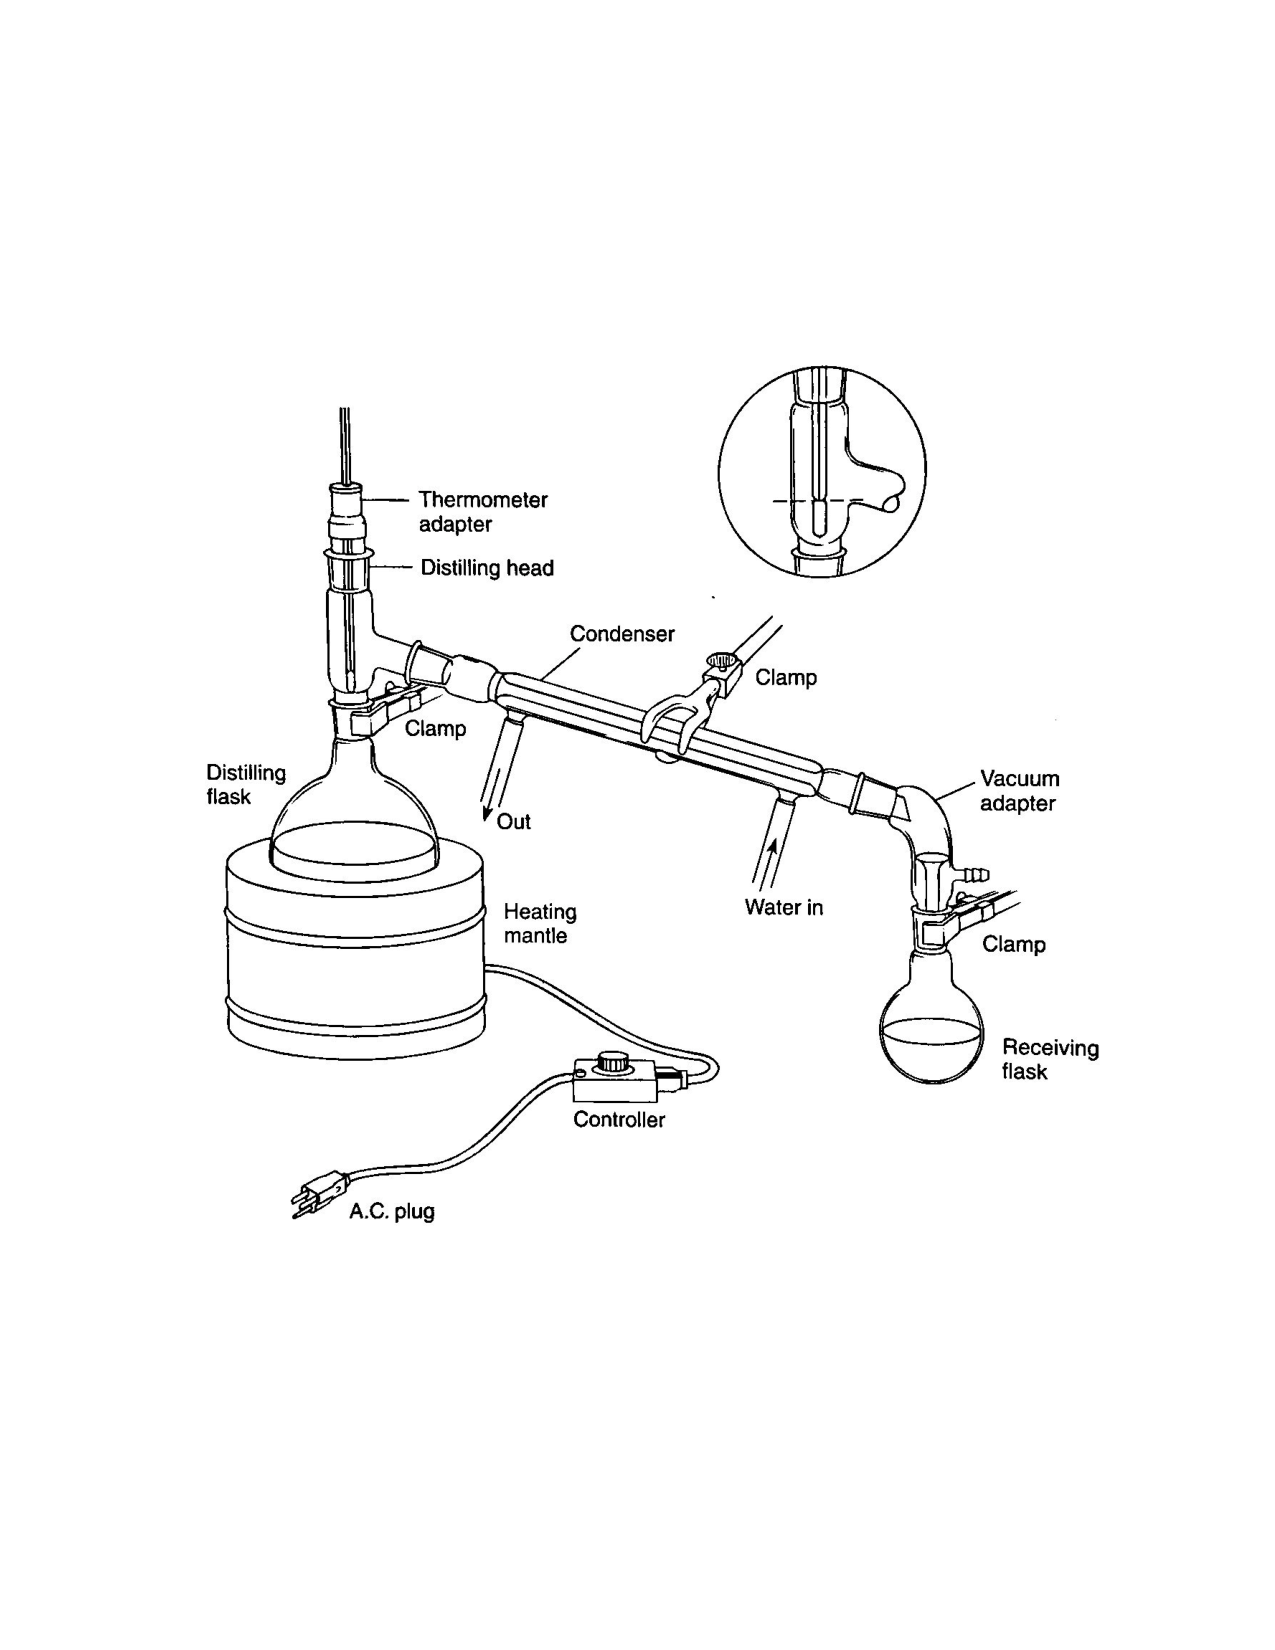
\includegraphics[width=0.95\textwidth]{figures/distillation_apparatus}
	\caption{A sample distillation apparatus. Note, your setup should use a two-neck flask for the distillation flask so the liquid samples can be pipetted out when necessary. Figure reproduced from \textcite{pavia1995organic}.}
	\label{fig:distillation_apparatus}
\end{figure}

A simple distilling apparatus that can be used for this experiment is shown in \cref{fig:distillation_apparatus}. 
The thermometer bulb should be approximately level with the side arm leading to the condenser, so the temperature measured reflects the vapor condensing down the tube. 
Except when samples of distillate are being taken for analysis, an adequate receiving flask should be placed at the lower end of the condenser. 

Before beginning the distillation, prepare twenty test tubes for taking samples. 
Write on the tubes the designations 1L, 1V, 2L, \dots, 10V (L=liquid residue; V=condensed vapor or distillate). 
The samples to be taken are approximately \qty{2}{\mL} in size. 

When the distillation is proceeding at a normal (not excessive) rate at about the desired temperature, quickly replace the receiver with a vial and read the thermometer. 
After about \qty{2}{\mL} has been collected, read the thermometer again, replace the receiver, and cork the vial tightly. 
Turn off and lower the heating mantle to halt the distillation. 
At the point where the temperature just begins to \emph{fall}, record another thermometer reading. 
After the flask has cooled \qtyrange{10}{20}{\celsius}, remove the stopper at the top of the flask and insert a \qty{2}{\mL} pipette equipped with a rubber bulb. 
Fill the pipette, discharge it into the appropriate test tube, and cork the flask. 

The following procedure is recommended for economical use of materials in carrying out this experiment. 
The paragraph numbers correspond to sample numbers. 
A graduated cylinder is adequate for measuring liquids. 
The temperatures recommended are those appropriate for an ambient pressure of \qty{1}{\atm}; at ambient pressures differing markedly from this, temperatures should be adjusted accordingly. 
\begin{enumerate}
	\item \textbf{Pure acetone} Introduce \qty{180}{\mL} of acetone into the flask. 
	Determine the boiling point by distilling to constant temperature.\sidenote{This temperature should be close to \qty{56.3}{\celsius} at \qty{1}{\atm}.}
	Collect samples (1V and 1L) for analysis if desired. 
	\item \textbf{Acetone-rich side of azeotrope, \qty[mode=text, reset-text-series=false]{58}{\celsius}} Cool the distilling flask and return the distillate removed in the previous step back to the flask. 
	Add \qty{20}{\mL} of chloroform to the flask. 
	Begin distillation. 
	When the temperature reaches \qty{\sim58}{\celsius}, collect about \qty{2}{\mL} of distillate (2V) and \qty{2}{\mL} of residue (2L).
	\item \textbf{\qty[mode=text, reset-text-series=false]{60}{\celsius}} Resume the distillation. 
	Take samples (3V, 3L) at \qty{\sim60}{\celsius}.
	\item \textbf{\qty[mode=text, reset-text-series=false]{62}{\celsius}} Resume the distillation and continue to around \qty{61}{\celsius}. 
	Cool the flask somewhat and add \qty{35}{\mL} of chloroform and \qty{65}{\mL} of acetone. 
	Resume the distillation.
	Take samples (4V, 4L) at about \qty{62}{\celsius}. 
	\item \textbf{\qty[mode=text, reset-text-series=false]{63.5}{\celsius}} Resume the distillation and continue to about \qty{63}{\celsius}. 
	Cool the flask somewhat and add \qty{50}{\mL} of chloroform and \qty{50}{\mL} of acetone. 
	Resume the distillation, saving the distillate for later use. 
	Take samples (5V, 5L) at about \qty{63.5}{\celsius}. 
	\item \textbf{Azeotrope} Resume the distillation and continue distilling until the boiling point ceases to change significantly, and take samples (6V, 6L).\sidenote{If the boiling point does not become sufficiently constant, analyze the remaining residue with the refractometer and make up \qty{100}{\mL} of solution to the composition thereby found. Distill this to constant temperature and take samples.}
	\item \textbf{Pure chloroform} Rinse the flask with a little chloroform. 
	Introduce \qty{80}{\mL} of chloroform and determine the boiling point the same way you did in step 1.
	\item \textbf{Chloroform-rich side of azeotrope, \qty[mode=text, reset-text-series=false]{62.5}{\celsius}} Cool the flask.
	Return the distillate of step 7 to the flask and add \qty{20}{\mL} of combined distillate and residue from steps 5 and 6. 
	Resume the distillation and take samples (8V, 8L) at about \qty{62.5}{\celsius}. 
	\item \textbf{\qty[mode=text, reset-text-series=false]{63.5}{\celsius}} Cool the flask, return the distillate from step 8, and add \qty{\sim50}{\mL} of the distillate and residue from steps 5 and 6. 
	Resume the distillation and take samples (9V, 9L) at around \qty{63.5}{\celsius}. 
	\item \textbf{Azeotrope\sidenote{We perform this step to verify the results from step 6.}} Resume the distillation, continue to constant boiling point, and take samples (10V, 10L). 
\end{enumerate}

At any convenient time after the samples have been taken, measure and record the index of refraction of each sample. 
If the experiment is being performed by several groups using the same refractometer, it is prudent to take samples to the refractometer as soon as six or eight samples are ready, or fewer if the instrument happens to available. 
If careful attention is given to the proper technique of using the refractometer, it should be possible to take readings at a rate of one sample per minute. 

At the end of the experiment, all acetone--chloroform mixtures should be poured into the designated waste container. 

At some point during the laboratory period, a barometer reading should be taken. 
The ambient temperature should be recorded for the purpose of making thermometer stem corrections. 

\section{Data Analysis}
\label{sec:data_analysis}

By interpolation in \cref{tab:ri_table}, convert the measured refractive indices to mole fractions. 
Plot the temperatures (after making any necessary stem corrections) against the mole fractions. 
Draw one smooth curve through the distillate points (V) and another through the residue points (L). 
Label all fields of the diagram to indicate what phases are present. 
Report the azeotropic composition and temperature together with the atmospheric pressure (\ie, the properly corrected barometer reading). 

\section{Lab Report Guidelines} % (fold)
\label{sec:lab_report_guidelines}

Your lab report should consist of the following parts:
\begin{description}
	\item[Title, Author and Date]
	\item[Introduction] Describe the experiment and expected results in a few sections. 
	\item[Experimental Theory] Reference this document.
	\item[Experimental Procedure] This should be a very brief general outline of the procedure, written out as a paragraph or two. Give the make and model for any major instruments you used, as well as any important settings. The description should be thorough enough that another student can repeat your experiments. This means you must provide explicit volumes, weights, and temperatures. Use the past tense in all of your descriptions. Don't just copy the procedure from the manual, state what work \emph{you} performed. 
	\item[Results and Discussion] This should include an overview of the analyzed data and responses to the questions worked into a natural narrative. 
	Include your data in a \emph{tabular} format, including all the information necessary to repeat your calculations. 
	Include all graphs as figures (with captions). 
	Your graphs should include axes labels (with units). 
	Discuss the \emph{chemical significance} of the results. 
	The chemical significance can be addressed in several alternate ways:
	\begin{itemize}
		\item State why these results are useful and important, or
		\item State how this experiment and technique fit into the larger world of chemistry, or
		\item Discuss why someone might need to perform a study of this type.
	\end{itemize}
	\item[References] Include any external material you incorporated into this report. 
	\item[Appendix] At the very end of your report, include examples of any calculations that you did by hand. 
	Include any additional files and code that you used to generate your graphs.
\end{description}
